\subsection{Components}

\note{Feel free to move and change the name of this subsection later}

This is my cool document. I have a lot of cool things to say. I was here. \note{note to self: Improve this introduction}

i can use citations too \cite{normal_distribution_wiki_page}.

\begin{figure}
    \begin{center}
    \begin{tikzpicture}[auto, node distance=2cm,>=latex']
        
        % Inputs
        % \node [input] (input_name) {};
        \node [input] (sensor_1) {};
        \node [input, yshift= 1cm] (sensor_2) {};
        \node [input, yshift= -1cm] (sensor_3) {};

        % Blocks
        % \node [block, location, node distance=xcm, minimum width=xcm] (block_name) {label};
        \node [block, right of=sensor_1, node distance=3cm, minimum width=2cm, minimum height=3cm] (RP2040) {RP2040};

        % Outputs
        % \node [output, location] (output_name) {};
        \node [output, right of=RP2040] (output) {};

        % Arrows
        % \draw [->] (point_A) -- node {label} (point_B);
        \draw [->] (sensor_1) -- ++ (2,0) node [near start, above] {load cell} (RP2040);
        \draw [->] (sensor_2) -- ++ (2,0) node [near start, above] {sap flow sensor} (RP2040);
        \draw [->] (sensor_3) -- ++ (2,0) node [near start, above] {leaf temp} (RP2040);

        \draw [->] (RP2040) -- node [near end, above] {output} (output);
            
    \end{tikzpicture}
    \end{center}
    \caption{Block of diagram of the system}
    \label{block_diagram}
\end{figure}

As seen in \cref{block_diagram} there were lots of blocks


SDI-12

\begin{figure}
    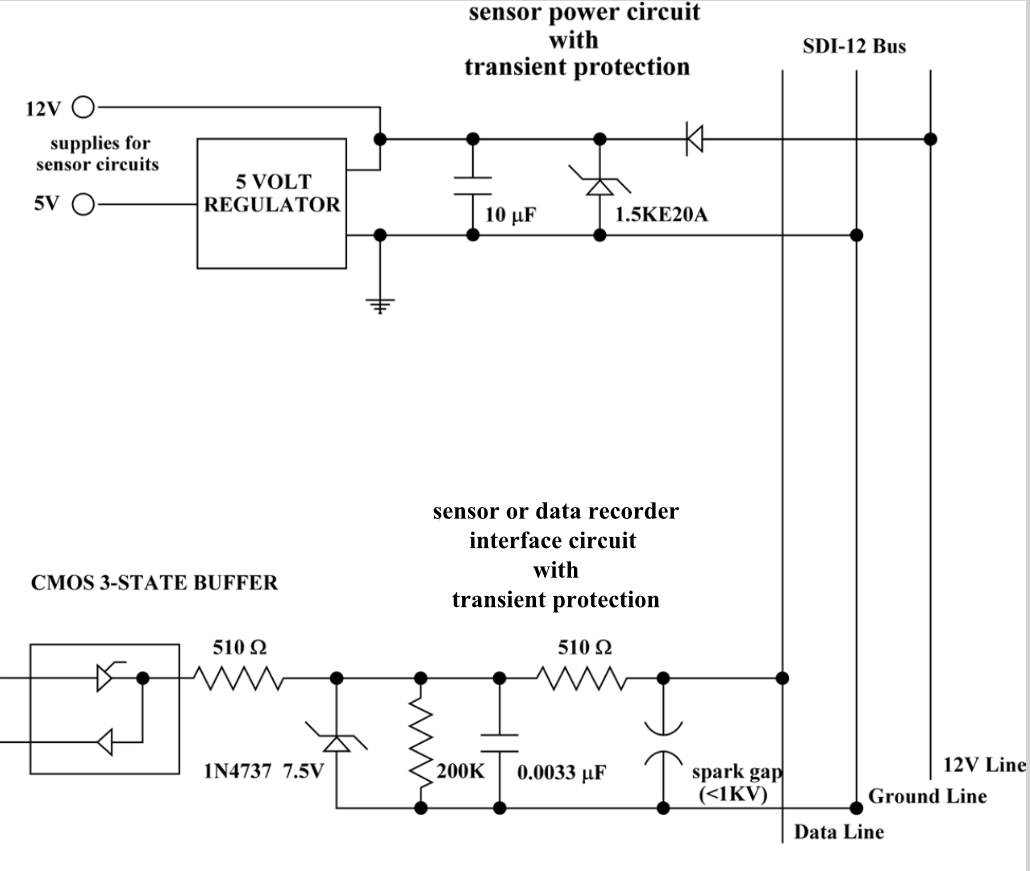
\includegraphics[width=\linewidth]{SDI-12 circuit.png}
    \caption{SDI-12 Circuit}
    \label{sdi12_circuit}
\end{figure}